\section{极化恒等式}
当出现向量点乘（如 $\overrightarrow{PA} \cdot \overrightarrow{PB}$ 时），我们最简单想到 $\overrightarrow{PA} \cdot \overrightarrow{PB} = |\overrightarrow{PA}| \cdot |\overrightarrow{PB}| \cdot \cos(\theta)$，然而，当 $P$ 点为动点时，$\overrightarrow{PA}$ 和 $\overrightarrow{PB}$ 的模长是变化的，$\theta$ 也在变化，这样就很难处理了。此时极化恒等式应运而生，它是为了消除 $\theta$ 的影响，变为仅与模长有关的式子。

\subsection{极化恒等式的定义}
\begin{definition}
    我们不妨取 $AB$ 的中点 $M$，可得 $\overrightarrow{PA} = \overrightarrow{PM} + \overrightarrow{MA}$，$ \overrightarrow{PB} = \overrightarrow{PM} + \overrightarrow{MB}$，根据中点，有 $\overrightarrow{MA} = -\overrightarrow{MB}$，则可以得到以下式子：
    \begin{align}
        \overrightarrow{PA} \cdot \overrightarrow{PB} & =(\overrightarrow{PM} + \overrightarrow{MA}) \cdot (\overrightarrow{PM} + \overrightarrow{MB}) = (\overrightarrow{PM} - \overrightarrow{MB}) \cdot (\overrightarrow{PM} + \overrightarrow{MB}) \\
                                                      & = |PM|^2 - |MB|^2 = |PM|^2 - \frac{1}{4}|AB|^2
    \end{align}
\end{definition}

\begin{multicols}{2}
    \begin{tikzpicture}[scale=0.7]
        \draw[thick] (0, 0) node[anchor=north east] {A} -- (4, 0) node[anchor=north west] {B} -- (2, 3) node[anchor=south] {P} -- cycle;

        % 绘制中点M
        \coordinate (M) at ($ (0,0)!.5!(4,0) $); % BC的中点
        \filldraw (M) circle (2pt) node[anchor=north] {M};

        \draw[->, thick, -{Stealth[length=4mm, width=2mm]}] (2,3) -- (M);
    \end{tikzpicture}

    \columnbreak

    可简记为：$\text{中线}^2 - \frac{1}{4}\text{底边}^2$

    注意上面提到的内容，\textbf{极化恒等式在动点问题中运用的是最频繁的}。

\end{multicols}

\subsection{三角形极化恒等式的运用}

\begin{example}
    在Rt $\triangle ABC$中，角$A, B, C$所对应的边为$a, b, c, A = \frac{\pi}{6}, C = \frac{\pi}{2}, c=2, P$是$\triangle ABC$外接圆上一点，则$\overrightarrow{PC} \cdot (\overrightarrow{PA} + \overrightarrow{PB})$的最大值是 ( \hspace{1.5cm} )
    \begin{tasks}(4) % (4) 表示每行4个选项
        \task 4
        \task $2+\sqrt{10}$
        \task 3
        \task $1+\sqrt{10}$
    \end{tasks}
\end{example}

\begin{example}
    在矩形$ABCD$中，$AB=2, AD=3, P$为矩形$ABCD$所在平面内的动点，且$PA=1$，则$\overrightarrow{PB} \cdot \overrightarrow{PC}$的最大值是 ( \hspace{1.5cm} )
    \begin{tasks}(4)
        \task 9
        \task 10
        \task 11
        \task 12
    \end{tasks}
\end{example}

\begin{example}
    如图，已知边长为4的正方形$ABCD$的中心与半径为$3\sqrt{2}$的圆$O$的圆心重合，点$P$是圆$O$上的一点，则$\overrightarrow{PA} \cdot \overrightarrow{PC} + \overrightarrow{PB} \cdot \overrightarrow{PD}$的值为 ( \hspace{1.5cm} )

    \begin{center}
        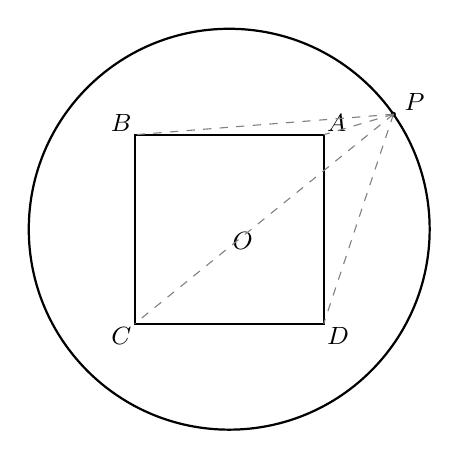
\begin{tikzpicture}[scale=0.6, % 调整图形的整体大小
                every node/.style={font=\small} % 统一设置节点字体大小
            ]
            % 定义圆心
            \coordinate (O) at (0,0);
            \node[below right, inner sep=1pt] at (O) {$O$}; % 标记圆心O

            \coordinate (A_pos) at (2,2);   % 右上角
            \coordinate (B_pos) at (-2,2);  % 左上角
            \coordinate (C_pos) at (-2,-2); % 左下角
            \coordinate (D_pos) at (2,-2);  % 右下角

            % 绘制正方形
            \draw[thick] (A_pos) -- (B_pos) -- (C_pos) -- (D_pos) -- cycle;

            % 标记正方形顶点 (使用 slightly more descriptive node names)
            \node[above right, inner sep=1pt] at (A_pos) {$A$};
            \node[above left, inner sep=1pt] at (B_pos) {$B$};
            \node[below left, inner sep=1pt] at (C_pos) {$C$};
            \node[below right, inner sep=1pt] at (D_pos) {$D$};

            % 圆的半径 R = 3*sqrt(2)
            % TikZ可以直接计算 sqrt(18) approx 4.2426
            \pgfmathsetmacro{\myCalculatedRadius}{3*sqrt(2)} % 计算并将结果存到 \myCalculatedRadius

            % 绘制圆
            \draw[thick] (O) circle (\myCalculatedRadius); % 使用计算的半径绘制圆

            % 点P在圆上，为了示意，我们取一个角度，例如25度，使其位置与图片类似
            % 图片中的P点在圆的右侧，略微偏上，靠近A和D的中垂线在圆上的交点
            \coordinate (P) at (35:\myCalculatedRadius); % P点在25度方向，半径为R的位置
            \node[above right, inner sep=1pt, xshift=1mm] at (P) {$P$}; % 稍微调整P标签位置避免遮挡
            \fill (P) circle (1.5pt); % 将P点画成一个小实心圆

            \draw[gray, thin, dashed] (P) -- (A_pos);
            \draw[gray, thin, dashed] (P) -- (B_pos);
            \draw[gray, thin, dashed] (P) -- (C_pos);
            \draw[gray, thin, dashed] (P) -- (D_pos);

        \end{tikzpicture}
    \end{center}

    \begin{tasks}(4)
        \task 16
        \task 20
        \task 28
        \task 32
    \end{tasks}
\end{example}

\subsection*{多选取值范围问题}

\begin{enumerate}[resume] % resume 会从上一个 enumerate 环境的计数继续

    \item 如图，$\triangle ABC$是边长为$2\sqrt{3}$的正三角形，$P$是以$C$为圆心，半径为$1$的圆上任意一点，则$\overrightarrow{PA} \cdot \overrightarrow{PB}$的取值可能是 ( \hspace{1.5cm} )
          \begin{center}
              \begin{tikzpicture}[scale=0.8]
                  % 定义正三角形边长
                  \pgfmathsetmacro{\sidelength}{2*sqrt(3)}
                  % 计算三角形的高
                  \pgfmathsetmacro{\triangleheight}{\sidelength*sqrt(3)/2} % h = s*sqrt(3)/2 = 3

                  % 定义顶点 C 在 (0, \triangleheight)
                  \coordinate (C) at (0, \triangleheight);
                  % 定义顶点 A 和 B，使 AB 在 x 轴上，中点为原点
                  \coordinate (A) at (-\sidelength/2, 0);
                  \coordinate (B) at (\sidelength/2, 0);

                  % 绘制三角形
                  \draw[thick] (A) node[below left] {$A$} -- (B) node[below right] {$B$} -- (C) node[above] {$C$} -- cycle;

                  % 绘制以 C 为圆心，半径为 1 的圆
                  \pgfmathsetmacro{\circleradius}{1}
                  \draw[thick] (C) circle (\circleradius);

                  % 在圆上取一个示意点 P (例如在左上方)
                  \coordinate (P) at ($(C) + (150:\circleradius)$); % 150度方向
                  \node[above left, inner sep=1pt] at (P) {$P$};
                  \fill (P) circle (1.5pt);

                  % (可选) 绘制向量 PA, PB
                  \draw[-latex, gray, dashed] (P) -- (A);
                  \draw[-latex, gray, dashed] (P) -- (B);
              \end{tikzpicture}
          \end{center}
          \begin{tasks}(4)
              \task 0
              \task 1
              \task 6
              \task 13
          \end{tasks}

    \item 如图，在$\triangle ABC$中，$AB \perp AC, \angle ABC = 30^\circ, AC=1, D$是$BC$的中点，$E$是以$B$为圆心，$BD$为半径的圆上任意一点，则$\overrightarrow{AD} \cdot \overrightarrow{AE}$的值可能为 ( \hspace{1.5cm} )
          \begin{center}
              \begin{tikzpicture}[scale=1.2]
                  % 已知条件
                  \def\AC{1}
                  \def\angleB{30} % 度

                  % 计算其他边长
                  % AB = AC / tan(B)
                  \pgfmathsetmacro{\AB}{\AC / tan(\angleB)} % AB = sqrt(3)
                  % BC = AC / sin(B)
                  \pgfmathsetmacro{\BC}{\AC / sin(\angleB)} % BC = 2
                  \pgfmathsetmacro{\BD}{\BC/2} % BD = 1 (半径)

                  % 定义顶点坐标
                  \coordinate (A) at (0,0);
                  \coordinate (C) at (0,\AC);
                  \coordinate (B) at (\AB,0);
                  % D是BC中点
                  \coordinate (D) at ($ (B)!0.5!(C) $);

                  % 绘制三角形ABC
                  \draw[thick] (A) node[below left] {$A$} -- (B) node[below right] {$B$} -- (C) node[above left] {$C$} -- cycle;
                  % 标记直角
                  \draw (A) + (0,0.2) -- + (0.2,0.2) -- + (0.2,0);

                  % 标记D点
                  \node[above right, inner sep=1pt] at (D) {$D$};
                  \fill (D) circle (1pt);

                  % 绘制以B为圆心，BD为半径的圆
                  \draw[thick] (B) circle (\BD);

                  % 在圆上取一个示意点 E (例如在圆的下方)
                  \coordinate (E) at ($(B) + (-70:\BD)$); % -70度方向
                  \node[below, inner sep=1pt] at (E) {$E$};
                  \fill (E) circle (1pt);

                  % (可选) 绘制向量 AD, AE
                  \draw[-latex, gray, dashed] (A) -- (D);
                  \draw[-latex, gray, dashed] (A) -- (E);
              \end{tikzpicture}
          \end{center}
          \begin{tasks}(4)
              \task $\frac{1}{2}$
              \task 1
              \task $\frac{5}{2}$
              \task 3
          \end{tasks}

    \item 已知正六边形$ABCDEF$的边长为4，$P$为正六边形所在平面内一点，则$\overrightarrow{PA} \cdot (\overrightarrow{PC} + \overrightarrow{PE})$的最小值为 \underline{\hspace{4cm}}.

    \item 如图，已知正方形$ABCD$的边长为2，若动点$P$在以$AB$为直径的半圆$E$（正方形$ABCD$内部，含边界）上，则$\overrightarrow{PC} \cdot \overrightarrow{PD}$的取值范围为 \underline{\hspace{4cm}}.
          \begin{center}
              \begin{tikzpicture}[scale=1]
                  \def\side{2} % 正方形边长

                  % 定义顶点
                  \coordinate (A) at (0,0);
                  \coordinate (B) at (\side,0);
                  \coordinate (C) at (\side,\side);
                  \coordinate (D) at (0,\side);

                  % 绘制正方形
                  \draw[thick] (A) node[below left] {$A$} -- (B) node[below right] {$B$} -- (C) node[above right] {$C$} -- (D) node[above left] {$D$} -- cycle;

                  % AB中点 (半圆圆心)
                  \coordinate (M) at ($ (A)!0.5!(B) $); % M is (1,0)
                  \pgfmathsetmacro{\radius}{\side/2} % 半径为1

                  % 绘制以AB为直径的半圆 (在正方形内部)
                  % 从M点，向左移动半径距离，开始画弧
                  \draw[thick] (M) ++(180:\radius) arc (180:0:\radius);

                  % 示意点P
                  \coordinate (P) at ($(M) + (60:\radius)$); % 例如在60度方向
                  \node[above] at (P) {$P$};
                  \fill (P) circle (1.5pt);
              \end{tikzpicture}
          \end{center}

    \item 如图，边长为2的菱形$ABCD$的对角线相交于点$O$，点$P$在线段$BO$上运动，若$\overrightarrow{AB} \cdot \overrightarrow{AO}=1$，则$\overrightarrow{PA} \cdot \overrightarrow{PB}$的最小值为 \underline{\hspace{4cm}}.
          \begin{center}
              \begin{tikzpicture}[scale=1.2]
                  \pgfmathsetmacro{\AO}{1}
                  \pgfmathsetmacro{\BO}{sqrt(3)}

                  % 定义顶点
                  \coordinate (O) at (0,0);
                  \coordinate (A) at (-\AO,0);
                  \coordinate (C) at (\AO,0);
                  \coordinate (B) at (0,-\BO);
                  \coordinate (D) at (0,\BO);

                  % 绘制菱形
                  \draw[thick] (A) node[left] {$A$} -- (B) node[below] {$B$} -- (C) node[right] {$C$} -- (D) node[above] {$D$} -- cycle;
                  \node[below left, inner sep=1pt] at (O) {$O$};

                  % 点P在线段BO上，示意
                  \coordinate (P) at ($ (B)!0.6!(O) $); % P在BO上，靠近O的60%处
                  \node[right, inner sep=2pt] at (P) {$P$};
                  \fill (P) circle (1pt);

                  % (可选) 绘制对角线
                  \draw[dashed, gray] (A) -- (C);
                  \draw[dashed, gray] (B) -- (D);
              \end{tikzpicture}
          \end{center}

    \item 已知正$\triangle ABC$的边长为2，点$P$为$\triangle ABC$所在平面内的动点，且$PC=1$，则$\overrightarrow{PA} \cdot \overrightarrow{PB}$的取值范围为 \underline{\hspace{4cm}}.

    \item 已知圆$O$的半径为2，$AB$为圆$O$的弦，弦长$AB=2, C$为圆$O$上任意一动点，则$\overrightarrow{AC} \cdot \overrightarrow{BC}$的取值范围是 \underline{\hspace{4cm}}.
\end{enumerate}

\subsection{大题的书写}

由于这是一个二级结论，在有用到极化恒等式的大题时，不能直接写 $$ = |PM|^2 - \frac{1}{4}|AB|^2 $$

我们需要熟背证明过程，照搬到答题卡上。

\pagebreak

\begin{enumerate}[label=\arabic*.] % 解答题从1开始编号
    \item 在四边形$ABCD$中，$\angle B=60^\circ, AB=4, BC=8,$且$\overrightarrow{AD}=\lambda \overrightarrow{BC}, \overrightarrow{AD} \cdot \overrightarrow{AB} = -4$.
          \begin{center}
              \begin{tikzpicture}[scale=0.5]
                  % 定义坐标点
                  \coordinate (B) at (0,0); % B 点
                  \coordinate (C) at (8,0); % C 点
                  \coordinate (D) at (4,4); % D 点（正上方）
                  \coordinate (A) at (2,4); % A 点（A 在 D 左侧）

                  % M, N 在 BC 上，按比例设置
                  \coordinate (M) at (2, 0); % M 点
                  \coordinate (N) at (5, 0); % N 点

                  % 绘制梯形 AB, CD
                  \draw[thick] (A) node[above] {$A$} -- (B) node[below left] {$B$} -- (C) node[below right] {$C$};
                  \draw[thick] (A) -- (D) node[above] {$D$} -- (C);

                  % 绘制 M 和 N，D 到 M、N 的连线
                  \node[below] at (M) {$M$}; \fill (M) circle (1.5pt);
                  \node[below] at (N) {$N$}; \fill (N) circle (1.5pt);
                  \draw[thick] (D) -- (M);
                  \draw[thick] (D) -- (N);

                  % 绘制角度标注
                  \draw pic[draw, "$\scriptstyle 60^\circ$", angle eccentricity=1.5, angle radius=0.5cm] {angle = C--B--A};

              \end{tikzpicture}
          \end{center}
          \begin{enumerate}[(1)]
              \item 求实数$\lambda$的值；
              \item 若$M, N$是线段$BC$上的动点，且$|\overrightarrow{MN}|=2$，求$\overrightarrow{DM} \cdot \overrightarrow{DN}$的最小值.
          \end{enumerate}

          \vspace{1cm}

    \item 如图，在$\triangle ABC$中，$D$是$BC$的中点，$E, F$是$AD$上的两个三等分点.

          \begin{tikzpicture}[scale=0.5]
              % 定义点的坐标
              \coordinate (B) at (0, 0); % B
              \coordinate (C) at (6, 0); % C
              \coordinate (D) at (3, 0); % D
              \coordinate (A) at (3.5, 7); % A

              % 绘制三角形和点
              \draw[thick] (B) node[below left] {B} -- (A) node[above] {A} -- (C) node[below right] {C} -- cycle;
              \draw[thick] (B) -- (D) node[below] {D};

              % 绘制连接 D、E 和 F 的线
              \coordinate (E) at ($(A)!1/3!(D)$);
              \coordinate (F) at ($(A)!2/3!(D)$);
              \draw[thick] (A) -- (E) node[pos=1.2, above right] {E};
              \draw[thick] (A) -- (F) node[pos=1.05, above right] {F};
              \draw[thick] (B) -- (E);
              \draw[thick] (C) -- (F);
              \draw[thick] (C) -- (E);
              \draw[thick] (D) -- (F);
              \draw[thick] (B) -- (F);
          \end{tikzpicture}

          \begin{enumerate}[(1)]
              \item 若 $AD = 5, BC = 4$, 求 $\overrightarrow{AB} \cdot \overrightarrow{AC}$;
              \item 若 $\overrightarrow{AB} \cdot \overrightarrow{AC} = 4, \overrightarrow{FB} \cdot \overrightarrow{FC} = -1$, 求 $\overrightarrow{EB} \cdot \overrightarrow{EC}$;
          \end{enumerate}
\end{enumerate}

\vspace{2cm}

\begin{ctt}
    至此，我们已经学会了使用极化恒等式。但并非所有向量点乘的形式都直接使用极化恒等式，这是一种不明智的选择，当出现夹角时，使用最基本的公式，还有一种情况，使用投影。接下来我们往下看。
\end{ctt}
